%\author{Grace Li}
%\author{Christopher Ing}
% \author{Dustin Little}
% \author{P. Lynne Howell}
% \email{howell@sickkids.ca}
% \affiliation[University of Toronto, Biochemistry]
% {Department of Biochemistry, University of Toronto, 27 King's College Circle, Toronto, Ontario, Canada M5S 1A1}
% \alsoaffiliation[Hospital for Sick Children]
% {Molecular Structure and Function, The Hospital for Sick Children, 555 University Avenue, Toronto, Ontario, Canada M5G 1X8}
% 
% \author{Mark Nitz}
% \email{nitz@chem.utoronto.ca}
% \affiliation[University of Toronto, Chemistry]
% {Department of Chemistry, University of Toronto, 80 St. George Street, Toronto, Ontario, Canada M5S 3H6}

%\author{R\'{e}gis Pom\`{e}s}
%\email{pomes@sickkids.ca}
%\phone{416 813 5686}
%\fax{416 813 5022}
%\affiliation[University of Toronto, Biochemistry]
%{Department of Biochemistry, University of Toronto, 27 King's College Circle, Toronto, Ontario, Canada M5S 1A1}
%\alsoaffiliation[Hospital for Sick Children]
%{Molecular Structure and Function, The Hospital for Sick Children, 555 University Avenue, Toronto, Ontario, Canada M5G 1X8}

\chapter[MD simulations of PgaB-glucosamine binding]{Molecular Dynamics simulations of PgaB and monosaccharides of N-acetyl-glucosamine}
% The contents of this section were adapted from an article published in the \emph{Journal of Physical Chemistry}.

\emph{Reference}: Part of this work is published in ``PgaB Contains a Carbohydrate Binding Domain Required for Modification and Export of Poly-$\beta$-1,6-N-acetyl-D-glucosamine"
\\
\\
\emph{Contributions}:
Grace Li conducted the MD simulation part of the research and wrote the section. Dustin Little conducted and interpreted the experimental results. Chris Ing parameterized the partial charges for glucosamine. R\'{e}gis Pom\`{e}s, Lynne Howell, Mark Nitz provided editorial input and guidance.

\newpage

\section{Summary}
% Note that this summary was taken from a draft of the paper written by Dustin from April 5th, 2013
%Bacteria embedded in a self-produced matrix of exopolymeric substance, or biofilm, are tolerant to antibiotics, protected from the environment, and isolated from the innate immune system. Production and de-N-acetylation of the exopolysaccharide poly-$\beta$-1,6-N-acetyl-D-glucosamine (PNAG) is important for biofilm formation in Escherichia coli. PgaB is essential for the partial de-N-acetylation of PNAG (dPNAG); a process required for polymer export and subsequent biofilm formation. Here we report 1.9 Å crystal structures of PgaB’s isolated C-terminal domain (PgaB-CT) and complex with glucosamine. The structure of PgaB-CT has structural difference from the previously reported PgaB42-655 structure (\textbf{What are these differences?}). Characterization of PgaB-CT using tryptophan fluorescence quenching assays shows binding to PNAG oligomers with ~1-4 mM affinity. These data in combination with molecular dynamics simulations of PgaB with N-acetylglucosamine and glucosamine suggest PNAG de-N-acetylation occurs first, with subsequent binding of dPNAG to the C-terminal domain. We believe this concerted action plays a pivotal role in targeting dPNAG for export through the outer membrane porin PgaA.
%
%From the book chapter XXX, PNAG is a homopolymer of beta(1,6) glcnac but with 20\% of the monomers deacetylated.  But then what would be the difference between dPNAG and PNAG? Or is it just a terminology difference between the two?

\section{Introduction}
% \textbf{In the second paper, experiments were performed to characterize the ability of PgaB-CT domain to bind carbohydrate substrates, which are short oligosaccharides of \pnag. The results of this study suggests a mechanism by which polymer substrates are bound and synthesized onto the protein.  Furthermore, a proposed mechanism of export is discussed.}

% \textbf{commentary: From reading what Dustin has written in the current introduction, I think their experimental data is quite weak.  Their key result is:  ``We show PgaB-CT binds PNAG oligomers with low affinity (what's the range?) using tryptophan fluorescence quenching, and have determined the structure of PgaB-CT in complex with glucosamine.'' I think MD simulations will be their best leverage for the proposed mechanism of export.}

% PgaB - description of the study, motivation and what has been done thus far
PgaB is a key protein responsible for the transport of the functionally relevant form of the exopolysaccharide poly-$\beta$-1,6-$N$-acetylglucosamine (PNAG) required for biofilm formation in a variety of pathogenic bacteria.\cite{Little:2012dp} The crystal structure of PgaB was recently solved in the laboratory of Dr. Lynne Howell.\cite{Little:2012dp} Structural and functional characterization have shown that PgaB is composed of two domains, an N-terminal de-N-acetylase domain, and a C-terminal domain with structural similarity to glycoside hydrolases.\cite{Little:2012dp}
% PgaB structure has been deposited in the PDB -- I did not find this June 30th 2012

Although it is known that PgaB functions by binding to PNAG, the molecular basis of the mechanism of export of PNAG by PgaB is currently not determined.  Moreover, the binding mode and the length of its substrate polymer are not known.
%PgaB binds PNAG or its de-N-acetylated end products, and what the  are. 
Efforts to crystallize PgaB with oligosaccharides of varying lengths have been impeded by the weak binding of short sugar polymers (eg. di- and tri-saccharides), and the insolubility of long sugar polymer chains (eg. those longer than a hexamer). However, molecular dynamics (MD) simulations are not impeded by these challenges and are well-suited for characterizing carbohydrate-protein interactions.\cite{Fadda:2010p5889}

% we examine putative binding site and modes of PNAG by examining the binding of GlcNAc and GlcNH2 monosaccharides with PgaB.
In this study, we perform atomistic MD simulations of PgaB with $\beta$-N-acetyl-glucosamine (GlcNAc) and protonated $\beta$-glucosamine (GlcNH$_{3}^{+}$), the monosaccharide components of the functionally-relevant polymer, dPNAG, to examine the putative binding site and binding modes of PNAG/dPNAG.  The weak binding affinity of these monosaccharides allows us to use a fragment-based methodology to probe for carbohydrate binding sites.  This method has been employed successfully in our previous studies to examine the binding mechanism of inositol, a carbohydrate-like amyloid inhibitor, with amyloidogenic peptides and their aggregates.\cite{Li:2012bx}
% Manuscript in preparation -- Li:2013Abreview
% \textbf{The objectives of this study are to (1) identify preferred binding sites of GlcNAc and glucosamine, (2) gain insight into the polymer directionality and (3) identify protein structural motions which may be correlated with ligand binding.}

% PgaB is hypothesized to bind sugar polymers (most likely a 15-mer) across its two domains on its surface. The polymer is hypothesized to extend out from the catalytic binding site (N-terminal domain) onto the charged grooves of the C-terminal domain.
% Experimentally it is known that shallow binding pockets exist at the surface of the proteins. REF?
% To our knowledge, this is the only study thus far in literature which employs large-scale MD simulations to predict carbohydrate-protein interactions. -- this is just not true.
% The objective of my work is to predict PNAG binding sites at the surface of PgaB using unrestrained molecular dynamics simulations in the presence of GlcNAc. This methodology was used in earlier inositol studies to predict inositol binding sites on amyloid peptides and aggregates.
% \textbf{The directionality of the polymer binding.  This is currently not experimentally determined.} 

\section{Material and Methods}
% Modelling details
A chimeric PgaB structure with the loop spanning residues 613 to 619 in the N-terminal domain modelled into the truncated crystal structure, was used in our simulations. The initial crystal structure has Ni$^{2+}$ bound at its enzymatic active site. Ni$^{2+}$ is octahedrally coordinated with surrounding residues and ligands.  The acetate ion bound to Ni$^{2+}$ near the active site, an artifact of crystallization, was removed in the simulation. Crystal waters were removed from the initial PDB structure. Histidine protonation states were assigned based on predicted pKa values using the web software PROPKA,\cite{Bas:2008ul,Olsson:2011vi,Sondergaard:2011ug} and histidine hydrogen-bonding geometries in the initial crystal structure.

Protein and ions were modelled using the AMBER99 force field.\cite{Cornell:1995td} Parameters for Ni$^{2+}$ were approximated using those of the magnesium ion (Mg$^{2+}$). After assigning protonation states of histidines, the net charge of the protein was -10e. The final simulation system comprised of 11 sodium (Na$^{+}$) counterions, and 45 molecules of free monosaccharride molecules (either GlcNAc or \glucosamine) at an effective concentration of 100 mM (Figure~\ref{fig:nag}). 19533 and 19991 water molecules were present in the GlcNAc and \glucosamine\ simulations, respectively. The initial volume of the simulation box is 713.6 nm$^{3}$.  To mimic experimental conditions, 100 mM of salt was added to the aqueous solution simulation systems containing \glucosamine.

% Note: To generate this structure from Glycam builder, choose the beta-pyranose ring and then acetyl-glucosamine
The structure of GlcNAc was generated using the web-based Glycam Biomolecule Builder.\cite{Woods:glycambuilder} The GLYCAM06 force field for carbohydrates\cite{Kirschner:2008ii} was used to model both GlcNAc and \glucosamine. A PDB of \glucosamine\ was obtained from the ZINC database.\cite{Irwin:2005kx} Energy minimization was performed using the software GAUSSIAN-09.\cite{g09} The minimized \glucosamine\ structure was consistent with the GLYCAM force field, and new RESP-derived partial atomic charges were computed for \glucosamine\ (a net charge of +1e) by fitting to a single HF/6-31G* molecular electrostatic potential (MEP) with a restraint weight of 0.01. MEPs were computed using the CHELPG methodology\cite{Breneman:1990ue} with the R.E.D. III software package.\cite{Dupradeau:2010bb} The partial charges were assigned so that the HCNH$_{3}$ group summed to a net charge of +1.164e, and the rest of the molecule summed to a net charge of -0.164e. Aliphatic hydrogen atoms were fitted with a zero partial charge for compatibility with GLYCAM06.
% How to cite the web builder - Carbohydrate Builder Woods Group. (2005-XXXX) GLYCAM Web. Complex Carbohydrate Research Center, University of Georgia, Athens, GA. (http://www.glycam.com) XXXX = current year

% Note put the partial charges used for glucosamine in an appendix. Ask Chris Ing to add to this methods description.

The TIP3P water model was used to represent the solvent. Version 4.5.5 of the GROMACS software package\cite{Pronk:2013ef,Hess:2008p5353} was used to perform unrestrained all-atom MD simulations with the stochastic dynamics algorithm using an integration timestep of 2 femtoseconds.

% Better organize below to make clear that I was using different integrators for equilibration and production dynamics.
% I still need to remind myself what rcoulomb and rlist corresponds to physically in the MD algorithm
Electrostatic interactions were calculated using Particle Mesh Ewald (PME) summation with a grid size of 0.12 nm and a Coulombic real-space cutoff of 1.1 nm. The Lennard-Jone potential was computed up to 1.2 nm using the GROMACS twin-range cutoff function with a short-range cut-off of 1.1 nm. Covalent bonds involving hydrogens were constrained using the LINCS algorithm. The simulation system was first subjected to energy minimization followed by a 1 ns equilibration in the NVT ensemble using Berendsen temperature coupling at 300 K with a coupling constant of 2.0.

A second equilibration was performed for 1 ns in the NpT ensemble with isotropic pressure coupling. Temperature and pressure for equilibration were controlled at 300 K and at 1 atm, respectively, using Berendsen thermostat and pressure coupling schemes. Production simulations were performed using the stochastic dynamics (sd) integrator and the Parrinello-Rahman barostat for pressure coupling.
% Look at /mnt/scratch_mp2/pomes/ligrace1/pgab/protein_sugar/params for fill in the blank parameters here

For each of GlcNAc and \glucosamine, 13 independent MD simulations at 130 ns per replica were performed, respectively, yielding a total of 3.38 $\mu$s of sampling time.

\subsection*{Analysis Protocol}
To compute spatial binding probability densities of GlcNAc and \glucosamine, frames from our simulations were first fitted via RMSD alignment of the protein backbone atoms to an energy minimized and MD-equilibrated crystal structure. The density map corresponds to the fractional atomic occupancy of GlcNAc or \glucosamine molecules binned using a grid with 1 \angstrom\ resolution.  The density map for each of GlcNAc and \glucosamine\ was computed using $\sim$165,000 time frames. The Visual Molecular Dynamics (VMD) software package\cite{Humphrey:1996to} was used to calculate and graphically render the densities depicted in Figures~\ref{fig:sdf}, \ref{fig:groove}, and \ref{fig:salt_density_distribution}.
% By examining the structure - does the sugars arrange into predicted binding site (s)?

\section{Results and Discussion}

%\subsection{Protein Dynamics}
%PgaB did not show any gross rearrangements or large perturbations during the simulations.
%RMSD of the entire protein
%RMSD of just the C-terminal domain
%Fluctuation of the loop region (Need a control simulation of just PgaB without any sugars).

\subsection{Comparisons of the binding modes of GlcNAc and \glucosamine}
% GlcNAc molecules preferentially bind to residues in the N-terminal domain (Figure~\ref{fig:pgab_density}B and D). 
% three main sites on PgaB (Figure~\ref{fig:pgab_binding_sites}). 
% Notably, the binding densities for GlcNAc (A, B in Figure~\ref{fig:pgab_binding_sites}A,B

The spatial binding probability density of GlcNAc, depicted in Figure~\ref{fig:sdf}, suggests that binding sites for GlcNAc are predominantly located in proximity to the active site (in the N-terminal domain), consistent with the function of PgaB as a PNAG de-acetylase. In particular, the densities in the inter-domain crevice beneath the loop spanning residue numbers 309 to 314 suggest that this region may be involved in substrate binding.  This result corroborates the hypothesis that the binding of PNAG to PgaB may initiate in this region, prior to binding at the active site.\cite{Little:2012dp} 

% Although the role of this region has not yet been determined experimentally
% in the inter-domain groove found directly beneath a loop connecting the two domains (Figure~\ref{fig:pgab_density}), and on the surface directly below the active site, which contains surface exposed hydrophobic residues.

% Moreover, our simulations have identified binding sites of GlcNAc that were not predicted from solely examining the static crystal structure. 

% When comparing the densities of PNAG and glucosamine (depicted in Figures \ref{fig:pgab_density} and XXX, respectively) it can be seen that whereas PNAG predominantly binds the N-terminal domain, but glucosamine instead bind to the C-terminal domain, predominantly in the groove capped by the loop spanning residues XXX to YYY.

By contrast, the spatial distribution of \glucosamine\ molecules depicted in Figure~\ref{fig:sdf} indicates that they preferentially bind to the C-terminal domain, with a significant density in the groove heavily lined with acidic and aromatic residues (Figure~\ref{fig:groove}).
%Specifically, glucosamine molecules are found to cluster in the groove lined with acidic, and aromatic residues (Figure~\ref{fig:groove}).  
Notably, consistent with the crystal structure of the C-terminal domain of PgaB (PgaB-CT) with bound \glucosamine, our simulation results indicate that both GlcNAc and \glucosamine\ possess binding sites at Trp613 and Trp552  (Figure~\ref{fig:groove}), which are conserved residues located in this groove.\cite{Little:2012dp}
%TODO get the correct reference for this.
% Trp613, Trp552 are in this groove
In support of this result, our previous study has shown that PgaB-CT is structurally similar to glycoside hydrolases,\cite{Little:2012dp} where the active site for these enzymes is also located in analogous grooves with a similar geometry. 

Furthermore, our results indicate that the entire length of the groove can bind \glucosamine\ molecules, suggesting that this groove is likely to accommodate a linear polymer of \glucosamine\ (Figure~\ref{fig:groove}). Accordingly, in our simulations, \glucosamine\ molecules were observed to bind in this groove by forming linear hydrogen-bonded chains (Figure~\ref{fig:directionality}).  Taken together,  our results suggest that this C-terminal groove of PgaB is a binding site for the de-acetylated PNAG (dPNAG).   In contrast to the spatial distributions of GlcNAc and \glucosamine, salt ions do not significantly bind the protein  (Figure~\ref{fig:salt_density_distribution}). 

Together, the morphology of the overall binding density of both GlcNAc and \glucosamine\ paints a molecular picture of the putative binding mechanism and export of PNAG. As PNAG is being shuttled through PgaB on to the next protein in the system, it initially binds at the cleft between the N- and C-terminal domains to reach the active site in order to undergo de-N-acetylation.  As it is converted to dPNAG, the binding affinity of the polymer is increased for the C-terminal domain, which can accommodate the de-acetylated portion of the substrate as it is being exported away from PgaB.

% Based on our results, GlcNAc may be more likely than glucosamine to bind at this loop binding site because the the binding densities for GlcNAc, but not for glucosamine persist at higher isovalues (0.2). -- Needs to be verified.

% This result further supports the ability of MD simulations and our methodology to identify carbohydrate-protein binding sites. 
% with the fact that these residues are conserved across PgaB  homologues. \textbf{See Dustin's first pgab paper} REF
% Notably, in our sim- ulations, glucosamine was found to adopt a binding mode consistent with the crystal structure
% Save this for the discussion section? Moreover, our simulations identified carbohydrate binding to Trp613, a key conserved residue across PgaB homologues that is found in the C-terminal domain loop spanning residues 613 to 619.
% TODO: Make a figure from MD showing glucosamine binding to compare to X-ray.
% TODO: Note that I should redo these plots with the correct density maps where I’ve correctly trjcatted the PgaB trajectories
% TODO: Note that here Kd calculations might help with hypothesizing which glcnac or glucosamine that binds there with high Kds.
% Because of the mobility of this loop region, we hypothesize that this loop may be involved in the export process whereby the opening and closing of this loop over the binding groove facilitate the export and stabilize the polymer for binding at the enzymatic active site.
% Loop clamping. Perhaps the loop may periodically open and clamp down (ie. bind particular sugars with higher affinity) on particular forms of the sugar on the PNAG.  It may clamp down for glucosamine or GlcNAc. 

% \textbf{I feel like this is really speculative, because its based on one snapshot - When a vector is drawn from the CX carbon to the nitrogen atom on the $NH_{3}^{+}$ group of glucosamine, we observe that these vectors point towards the N-terminal domain. Based on this result, we speculate that the (reducing or non-reducing end of the polymer?) to (reducing/non-reducing) end of the polymer extends from the N-terminal towards the C-terminal of PgaB.  This hypothesized polymer directionality is consistent with our proposed mechanism of synthesis and export whereby de-acetylation in PgaB-NT occurs prior to the binding of de-acetylated-PNAG by PgaB-CT.  Note that the hydrogen-bonded chain spanning the first three monomers in the groove shown in Figure~\ref{fig:} mimics the linkage pattern of PNAG, except you would have to rotate the schematic of PNAG by 180 degrees. See PNAG clipped from Little 2012, Figure S7.}

% I don't fully understand the directionality business.  Here is a hack job at summarizing what it is from readings.
% From wikipedia -- An oligosaccharide has both a reducing and a non-reducing end. The reducing end of an oligosaccharide is the monosaccharide residue with hemiacetal functionality, thereby capable of reducing the Tollens’ reagent, while the non-reducing end is the monosaccharide residue in acetal form, thus incapable of reducing the Tollens’ reagent.[2] The reducing and non-reducing ends of an oligosaccharide are conventionally drawn with the reducing-end monosaccharide residue furthest to the right and the non-reducing (or terminal) end furthest to the left.[2]

% directionality paper
% http://www.jbc.org/content/274/37/26557.full

This study demonstrates the utility of large-scale MD simulations in predicting carbohydrate-protein binding modes when combined with a force field that can reproduce sugar-protein interactions with relative accuracy (for example, GLYCAM\cite{Kirschner:2008ii}). Force fields for molecular simulations of carbohydrates have been recently reviewed here.\cite{Fadda:2010p5889}  Furthermore, we demonstrated the utility of computing spatial probability binding densities using monosaccharides to map carbohydrate binding sites. A recent study suggests that by building 3D density binding maps of carbohydrates and using this data with additional computational algorithms can increase the accuracy of identifying putative carbohydrate binding sites.\cite{Tsai:2012bj} As part of future work, it may be interesting to employ a similar approach to investigate the binding of oligosaccharides to PgaB.  

%%%%%%%%%%%%%%%%%%%%%% Future work %%%%%%%%%%%%%%%%%%%%%%
% What is the name for positively charged glucosamine molecules? Is there a 3-letter abbrev. for it?
% This paragraph can be part of the discussion.

% Various analyses (eg. time evolution of RMSD, RMSF of the protein, principle component analysis, etc.) can be done to quantify protein dynamics, especially the mobility of the two domains. Furthermore, it will be interesting to investigate how dynamics may be correlated to the function of PgaB.  Finally, it will be interesting to predict GlcNAc and GlcNH$_3^+$ binding modes and binding constants from MD simulations so that they can be compared with corresponding future experimental results.

% \subsection{New written up results to incorporate}
% These are results -- writing them here first 
% GlcNAc binding. Moreover, GlcNAc interacts with conserved hydrophobic residues X, Y, Z in CE4 (Figure S1 in Little, JBC, 2012). Figure caption (overlapped zoomed out densities): The magenta colored densities over PgaB-NT cover conserved residues in CE4.  These residues are highlighted in magenta in Little et. al. in Figure S1. 

% \subsection{From dustin's committee report (Jan 2013)}
% Significant efforts to obtain a co-crystal structure of PgaB (or PgaB-CT) in complex with a PNAG oligomer have failed.
% Description of glucosamine binding site on CT domain: This hypothesis (CT is a CBM) is further supported by a co-crystal structure of PgaB-CT in complex with glucosamine (Figure 4). Attempts to obtain PgaB-CT in complex with N-acetylglucosamine (GlcNAc) under equivalent crystallization conditions have been unsuccessful. PgaB-CT crystallized in the presence of 200 mM glucosamine yielded two large peaks (3?) in the unbiased |Fo – Fc| difference electron density map. The two density peaks could not be accounted for by side chain or buffer molecules, and were large enough to accommodate a glucosamine molecule. The first molecule of glucosamine was refined unambiguously and is coordinated by Asp472 and Trp552 (Figure 4). The second molecule was refined ambiguously keeping stereochemistry in the most preferred orientation, and is coordinated by Tyr432, Asp466, and Trp613 (Figure 4)

\section{Acknowledgements}
This work was done in collaboration with Dustin Little, Dr. Lynne Howell and Dr. Mark Nitz.

\section{Figures}

\begin{figure}[htbp]
\centering
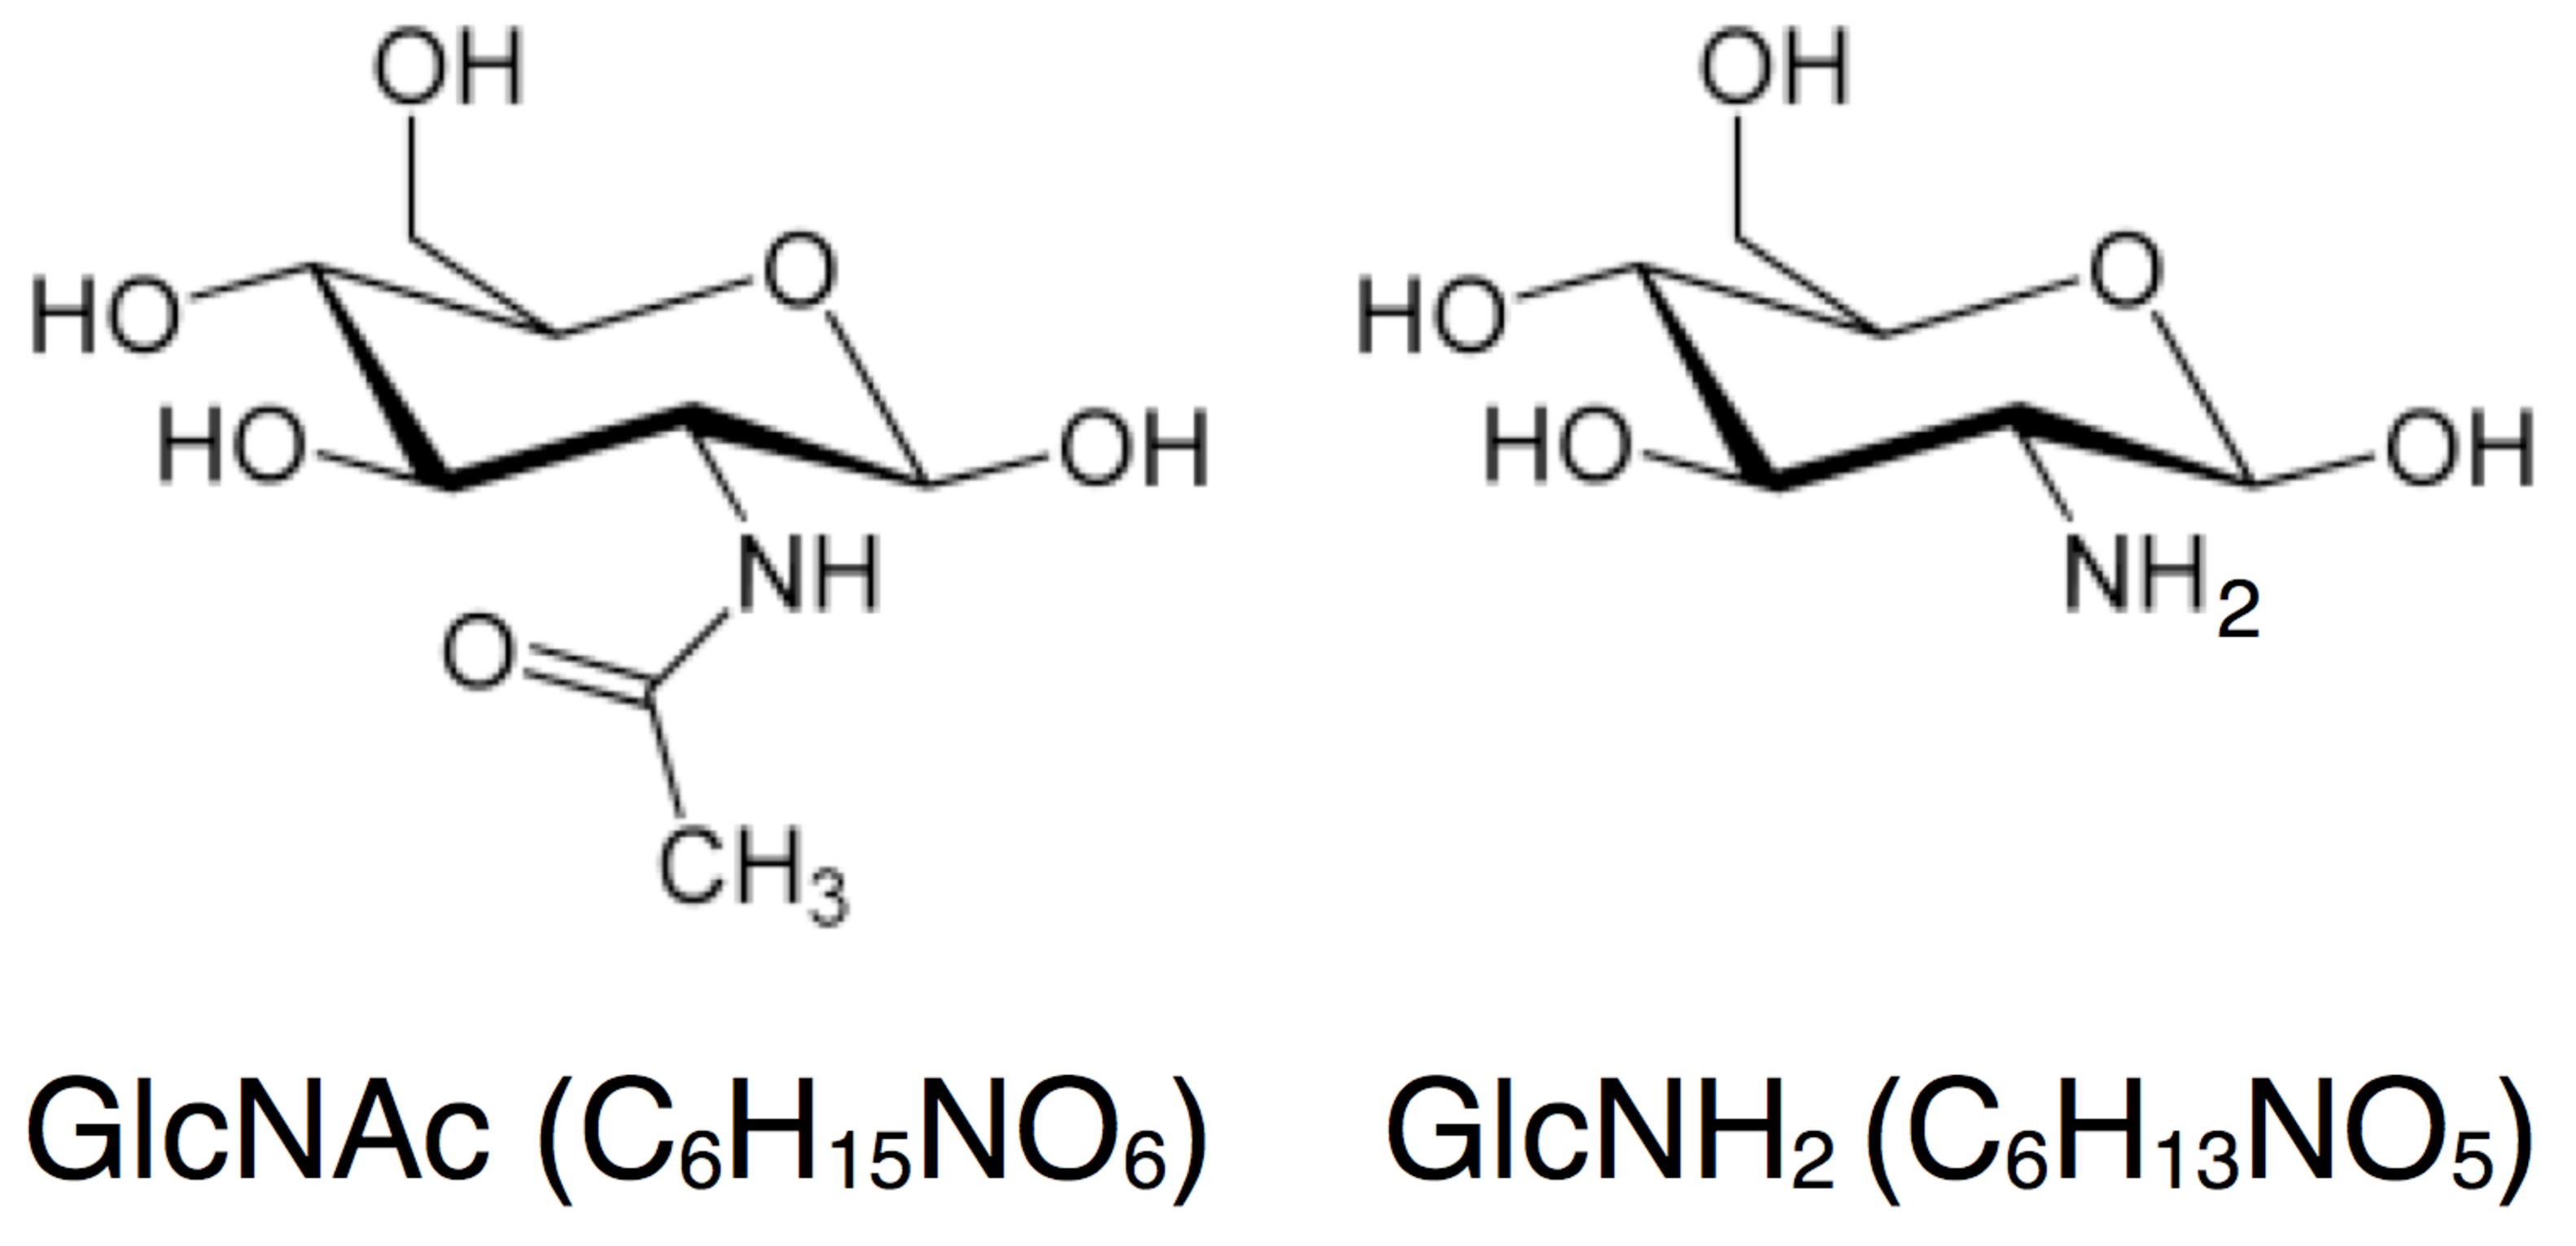
\includegraphics[width=4in]{figures/results4/sugar_structures.pdf}
\caption[Molecular structures of GlcNAc and GlcNH$_2$]{Molecular structures of $\beta$-N-acetyl-glucosamine (GlcNAc) and $\beta$-glucosamine (GlcNH$_2$).}
\label{fig:nag}
\end{figure}

%\begin{figure}[htbp]
%\centering
%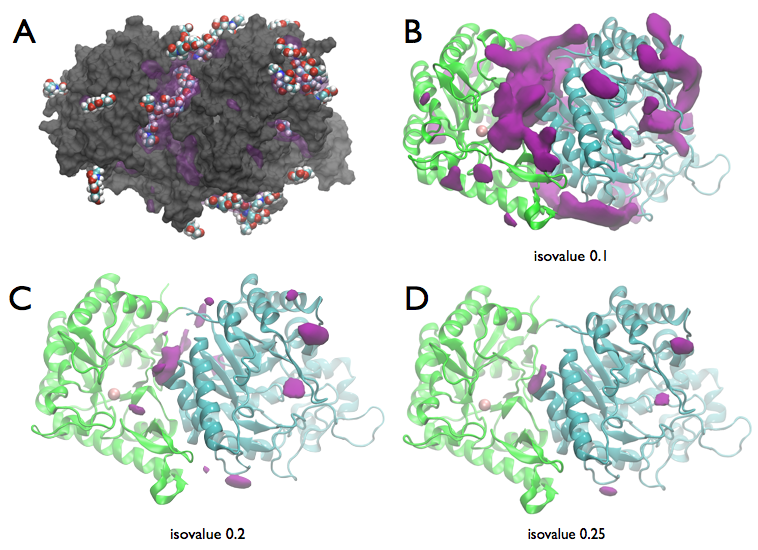
\includegraphics[height=4.25in, width=6in]{figures/results4/figure_pgab_density.png}
%\caption[NAG binding density]{Spatial binding probability density map of bound GlcNAc around PgaB.  (A) An example snapshot of PgaB (grey) shown using a surface representation with bound GlcNAc binding density depicted in purple at 10\% occupancy (iso-contour of 0.1). Binding densities of GlcNAc overlapped with a cartoon representation of PgaB at iso-contour levels of (B) 0.1 (C) 0.2 (D) 0.25. In our coloring scheme, residue numbers 43 to 310 and numbers 311 to 667 represent N- (green) and C-terminal (cyan) domains, respectively.}
%\label{fig:pgab_density}
%\end{figure}

%\begin{figure}[htbp]
%\centering
%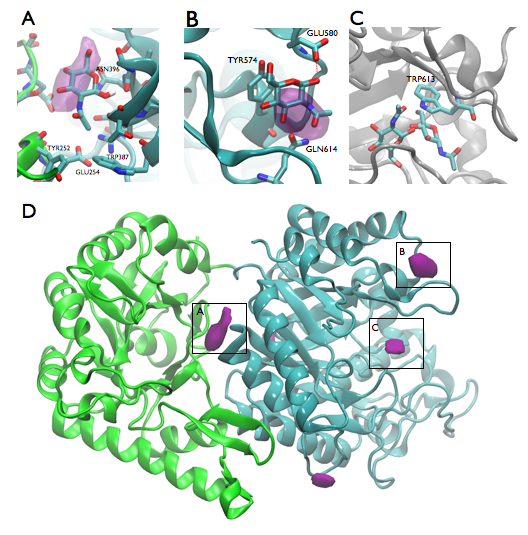
\includegraphics[height=6.29in, width=6.12in]{figures/results4/figure_pgab_binding_sites.png}
%\caption[GlcNAc binding sites]{High probability GlcNAc binding sites at an iso-contour value of 0.25 (D). Insets (A to C) show detailed views of the binding sites and the residues involved in binding. \textbf{This figure probably isn't that useful}}
%\label{fig:pgab_binding_sites}
%\end{figure}

\begin{figure}[htbp]
\centering
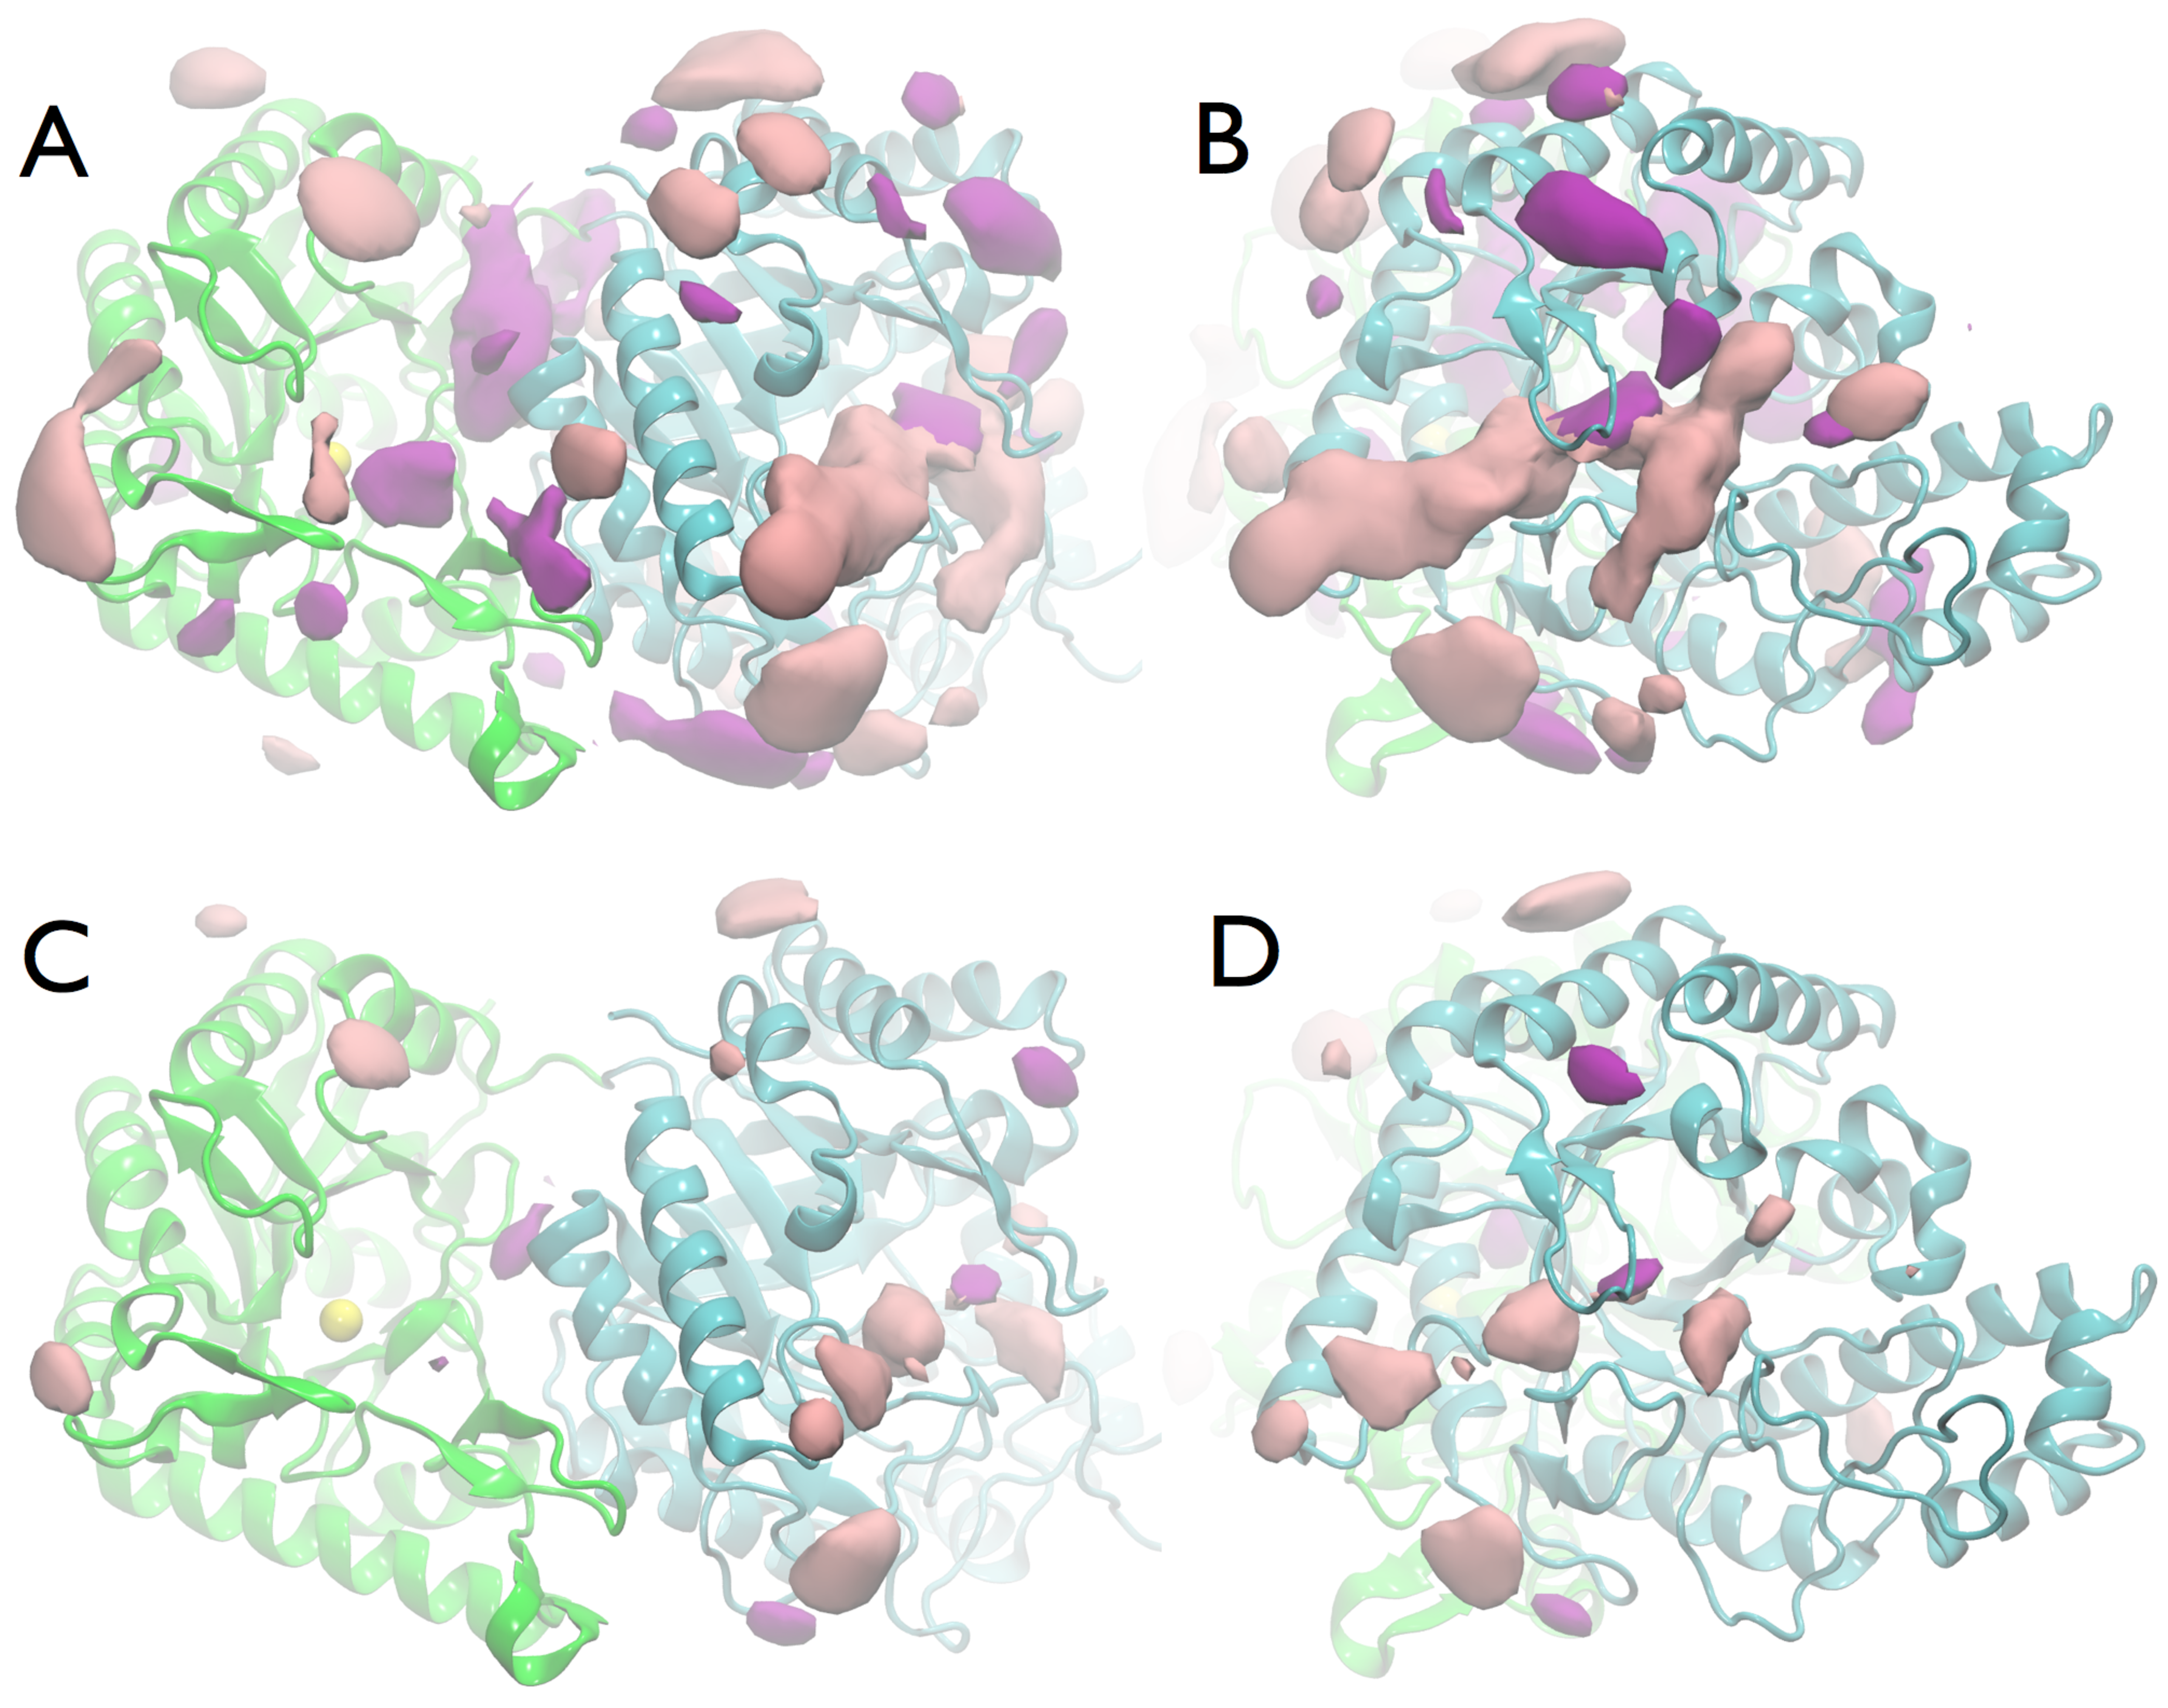
\includegraphics[width=6.25in]{figures/results4/glcnac_glucosamine_merged_sdf.pdf}
\caption[Spatial probability densities of bound GlcNAc (purple) and \glucosamine]{Spatial probability densities of bound GlcNAc (purple) and \glucosamine\ (pink).  Binding densities overlapped with a cartoon representation of the energy minimized crystal structure of PgaB.  The protein is shown facing the active site in (A) and (C), and shown facing the C-terminal domain in (B) and (D). In each view, binding densities are depicted at occupancies of 0.15 in (A)-(B), and 0.25 in (C) - (D). In our coloring scheme, residue numbers 43 to 310 and numbers 311 to 667 represent N- (green) and C-terminal (cyan) domains, respectively.}
% Note that the magenta colored densities over PgaB-NT cover conserved residues in CE4.  (These residues are highlighted in magenta in Little et. al. in Figure S1. ) \textbf{Id the residues and list them in the text and in the caption. Need to add the isovalues for the top and bottom two panels.}
\label{fig:sdf}
\end{figure}

\begin{figure}[htbp]
\centering
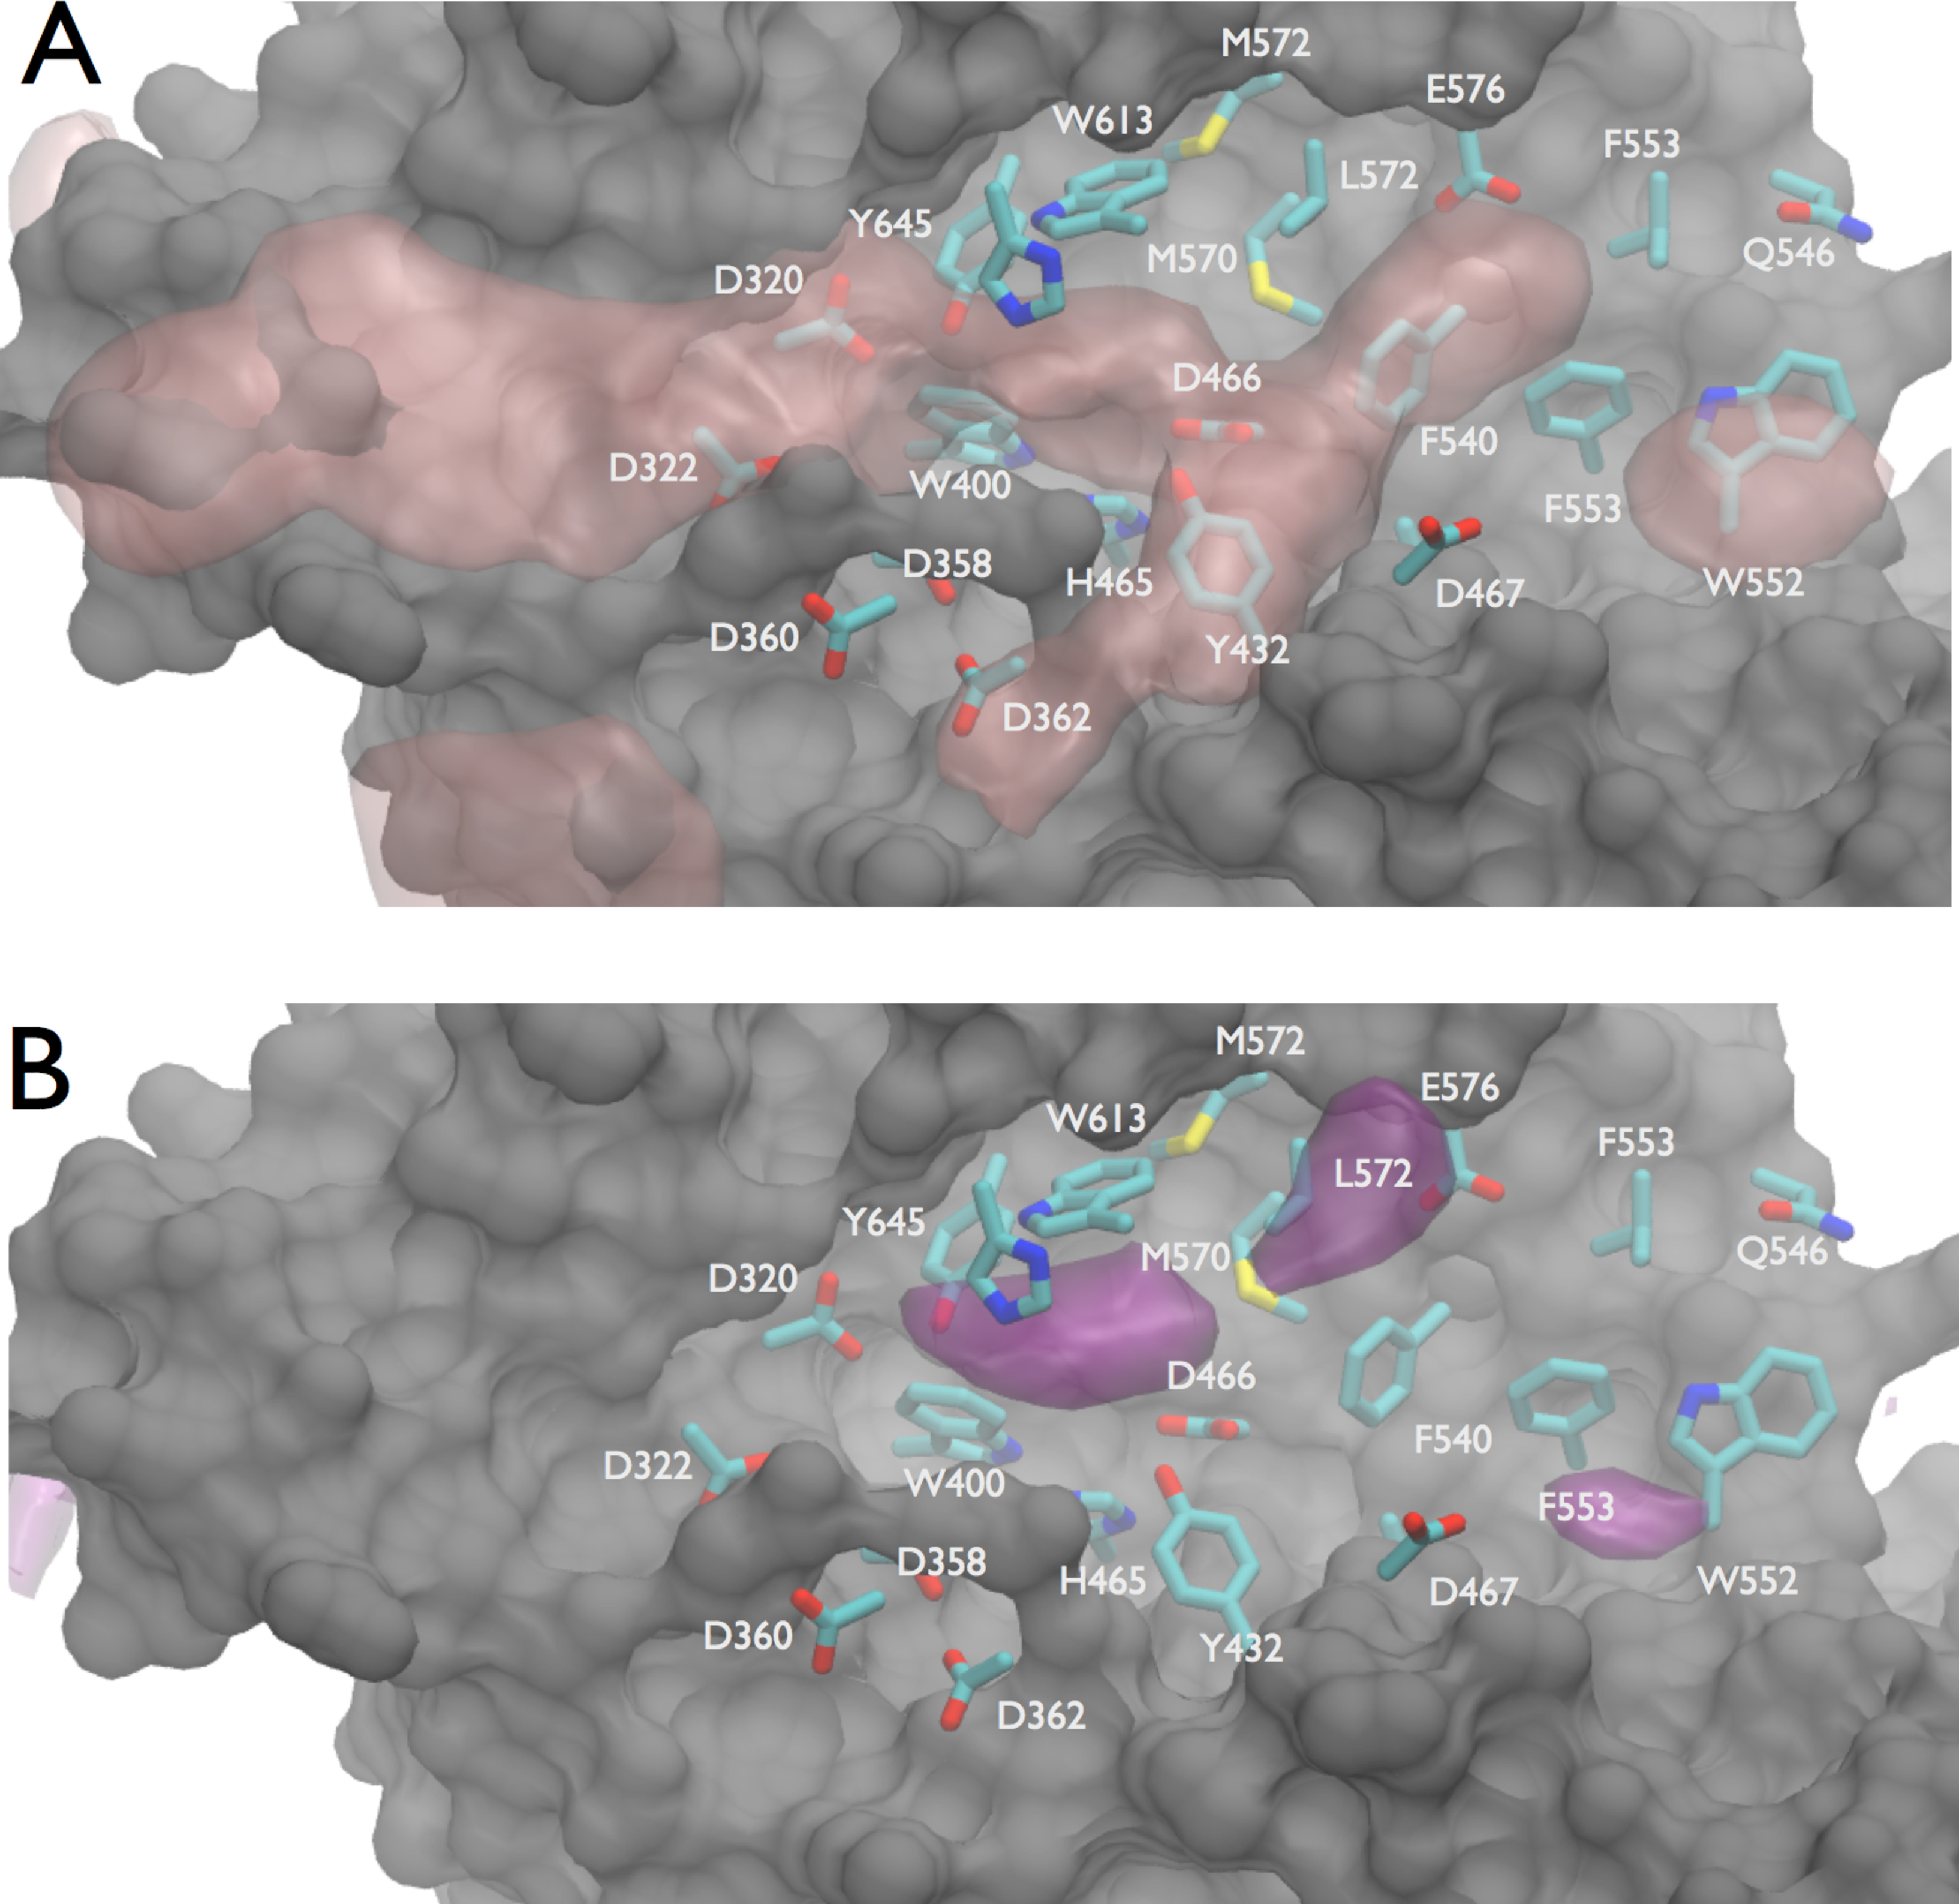
\includegraphics[width=6.25in]{figures/results4/cterm_groove_surf2.pdf}
\caption[Spatial probability densities of GlcNAc and GlcNH3+ in the C-terminal groove]{Spatial probability distribution shown at an occupancy of 0.15 for (A) \glucosamine\ and (B) GlcNAc in the binding groove of the C-terminal domain.  The residues in the groove are shown in stick representations.}
\label{fig:groove}
\end{figure}

\begin{figure}[htbp]
\centering
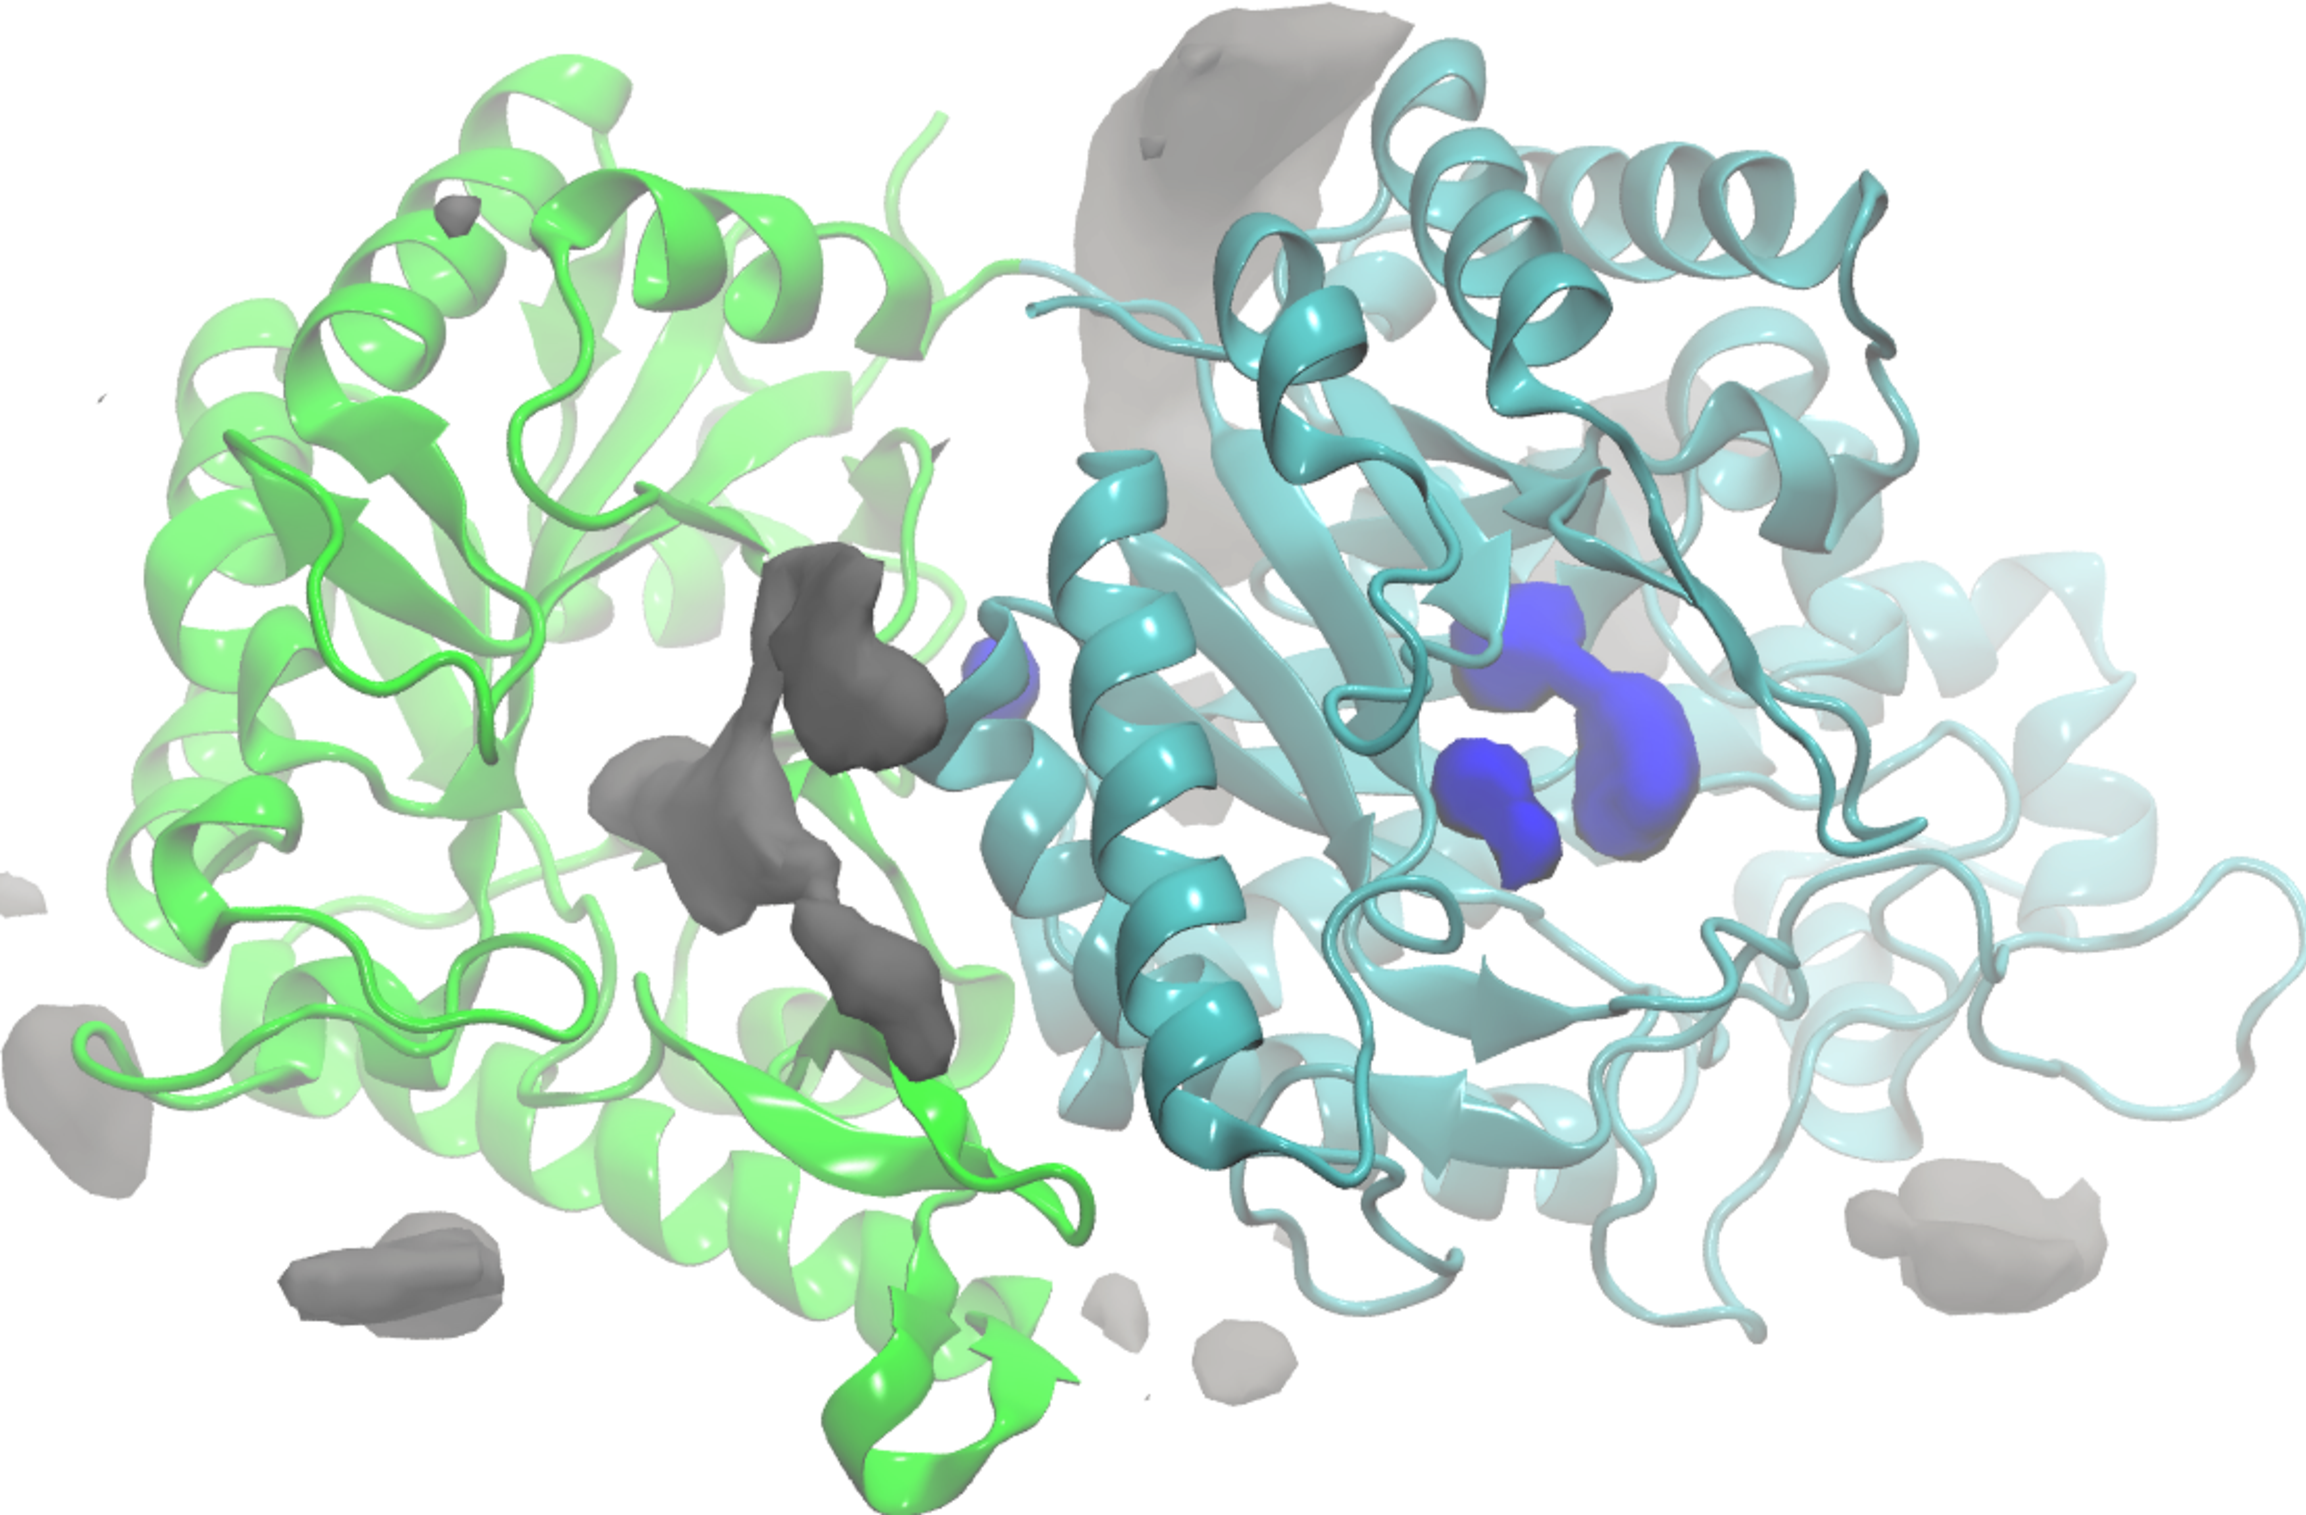
\includegraphics[width=6.25in]{figures/results4/pgab_glucosamine_salt_densities.pdf}
\caption[Ionic distribution]{Spatial probability distribution of sodium (blue) and chloride (grey) ions depicted at an isovalue of 0.005. The protein is depicted in a cartoon representation, with N- and C-terminal domains colored in green and cyan, respectively.}
\label{fig:salt_density_distribution}
\end{figure}

\begin{figure}[htbp]
\centering
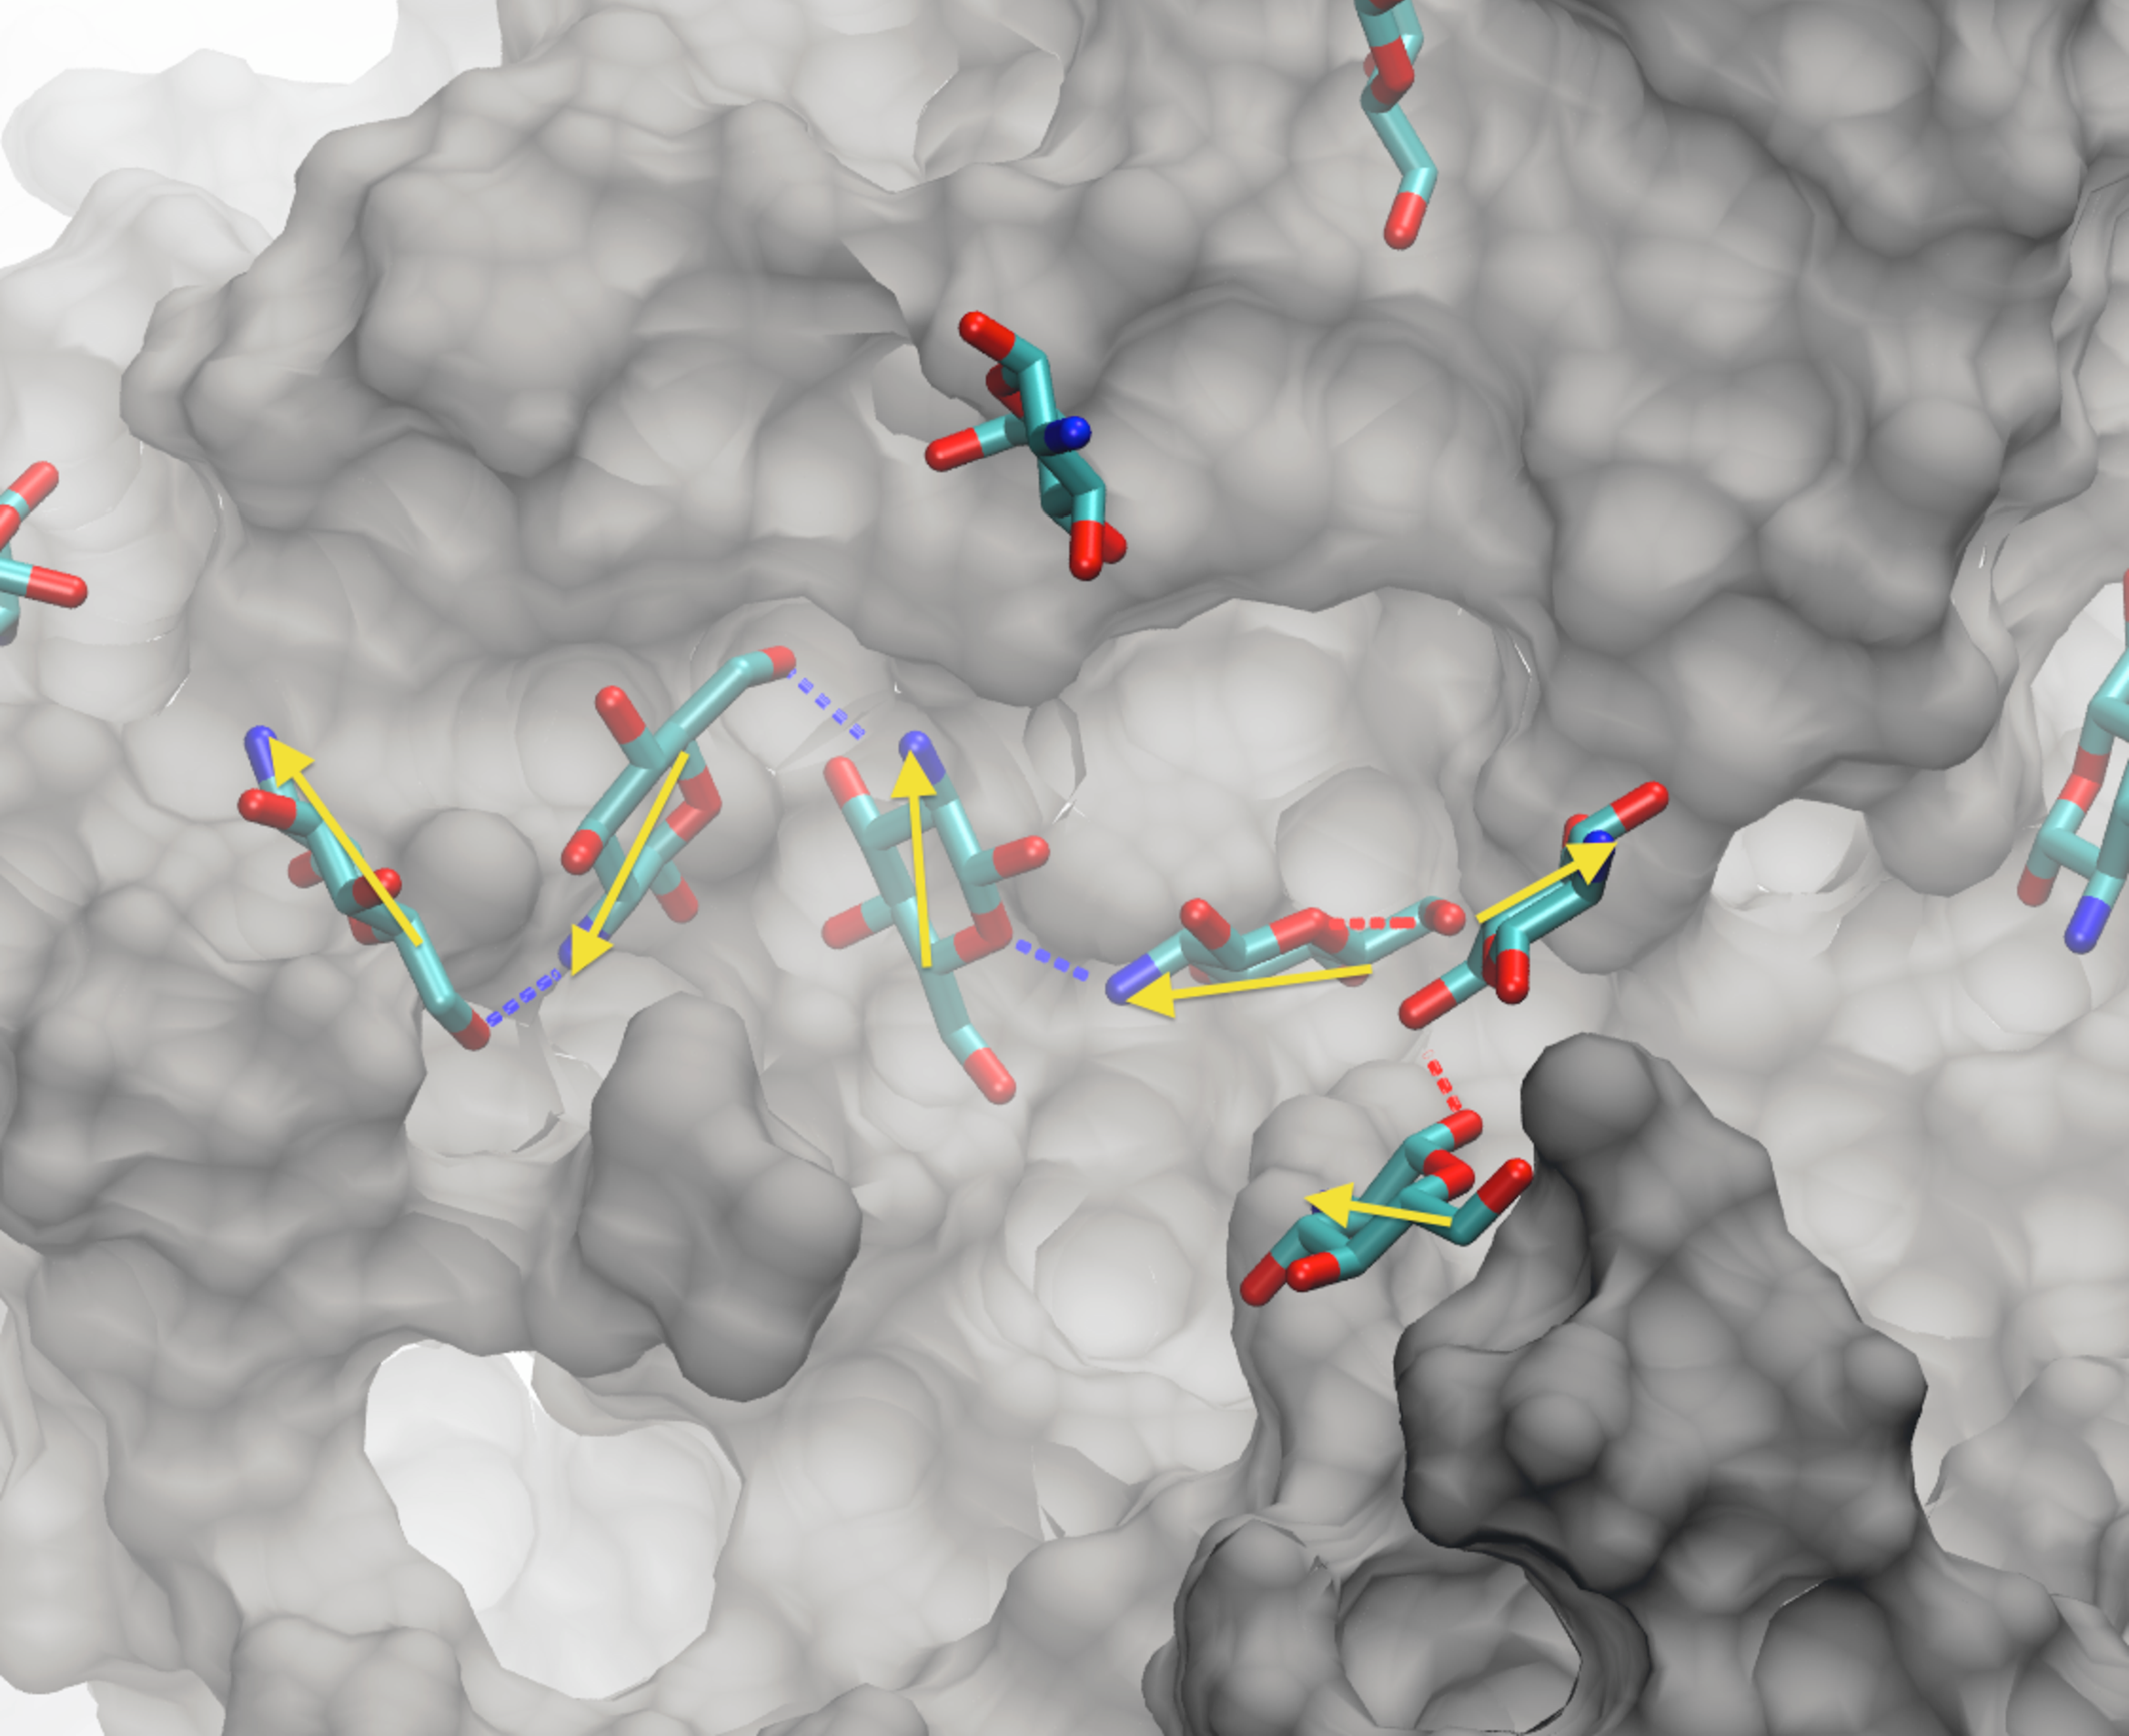
\includegraphics[width=6.25in]{figures/results4/glucosamine_binding_direction_suggestive.pdf}
\caption[Polymer directionality]{A linear chain of hydrogen-bonded \glucosamine\ molecules in the putative carbohydrate-binding groove of the C-terminal domain.  The yellow arrows are drawn as a guide to highlight a putative chain directionality.}
\label{fig:directionality}
\end{figure}

\begin{singlespace}
\addcontentsline{toc}{section}{Bibliography}
\bibliographystyle{elsart-num}
\bibliography{/Users/grace/github/thesis/document/results4/results4}
\end{singlespace}

% Objective of this work: 
% Binding surface - Map out a binding surface for both domains - We don't know what the C-Terminal domain is responsible for.  
% Compare and predict binding affinities.  Dustin is trying to get experimental data and co-crystal structures.

% Dustin -- But to get back to your main idea - i'm blabbering on here, other then the density map and binding constants. I guess it would be nice to see where the most flexible parts of the protein are - and what this might correlate too. What other quantitative values can you obtain?

% protein motion -- dynamics of the protein - can it be related to how it might function?
% \begin{itemize}
% 	\item Rmsd vs. time for the entire protein
% 	\item Rmsd vs. time for each of the individual domains
% 	\item Rmsf of the protein
% \end{itemize}

% % FIGURE
% \begin{figure}[pgab_rmsd]
% \centering
% 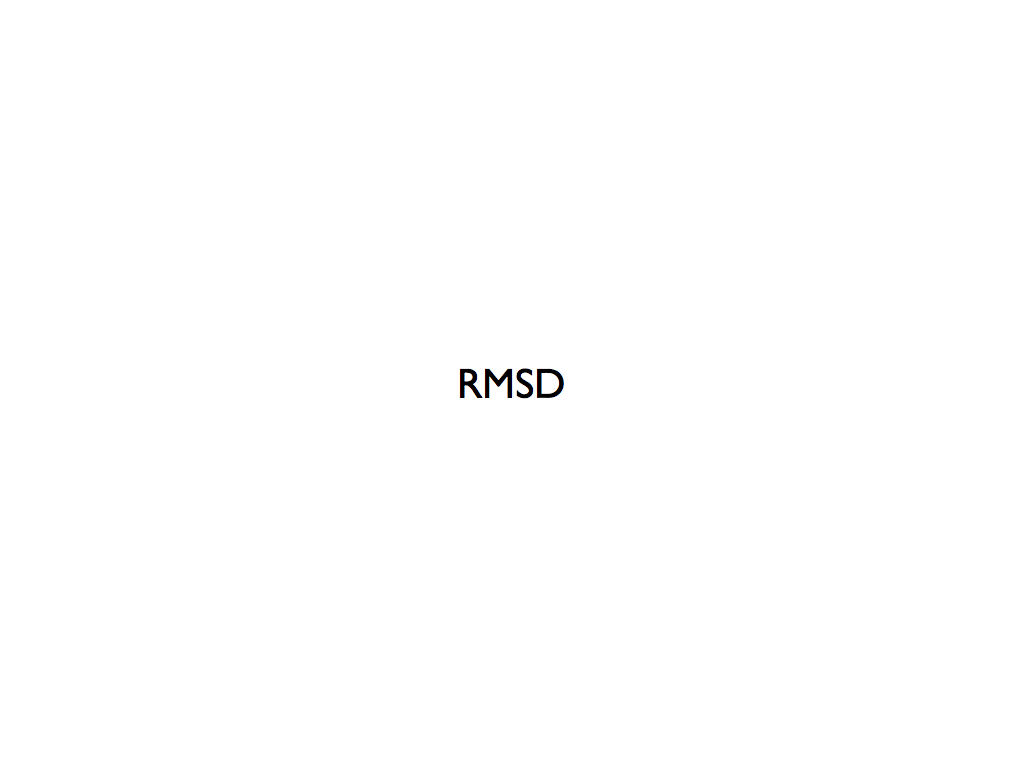
\includegraphics[height=4.1in, width=6.23in]{figures/pgab_rmsd.jpg}
% \caption[PgaB protein dynamics]{Time evolution of RMSD of PgaB from its crystal state}
% \label{fig:pgab_rmsd}
% \end{figure}
% 
% % FIGURE
% \begin{figure}[pgab_rmsf]
% \centering
% 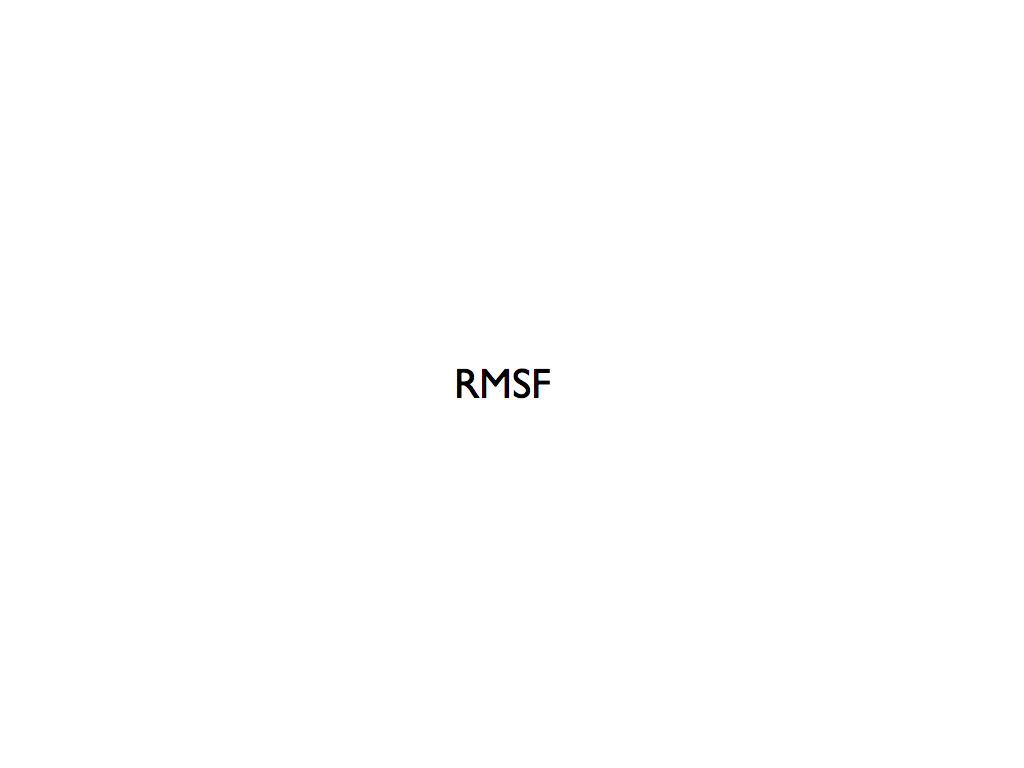
\includegraphics[height=4.1in, width=6.23in]{figures/pgab_rmsf.jpg}
% \caption[PgaB protein dynamics]{Time evolution of RMSD of PgaB from its crystal state}
% \label{fig:pgab_rmsf}
% \end{figure}

% FIGURE
% \begin{figure}[pgab_domains]
% \centering
% 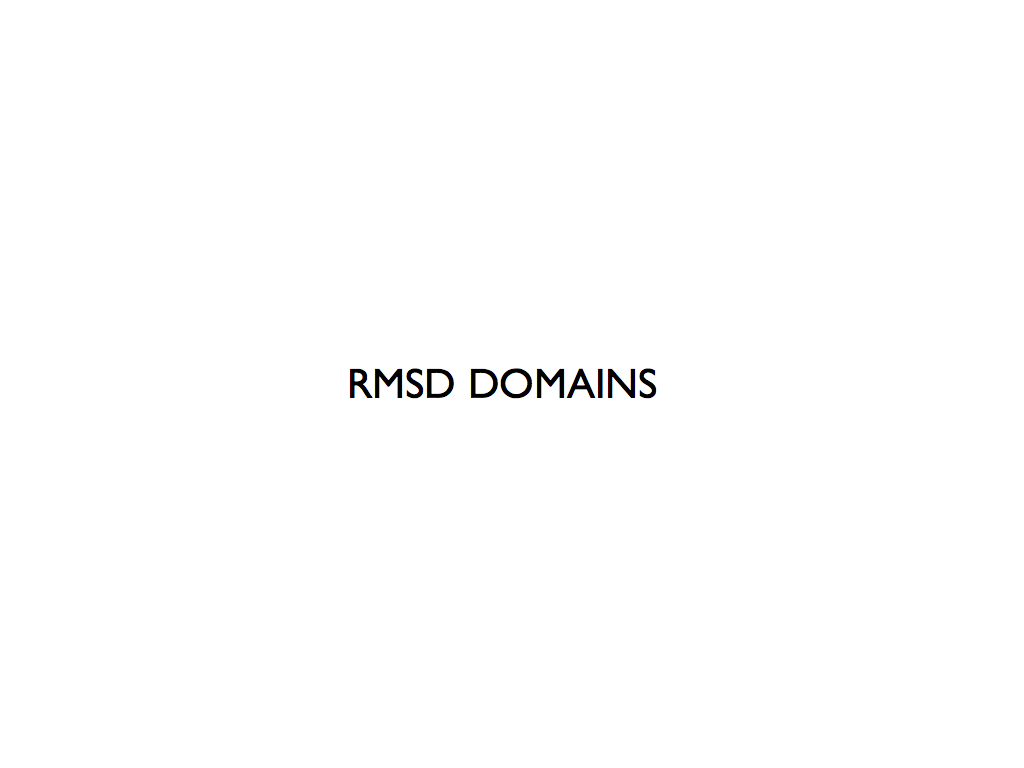
\includegraphics[height=4.1in, width=6.23in]{figures/pgab_domains.jpg}
% \caption[PgaB protein dynamics]{Time evolution of RMSD of PgaB from its crystal state}
% \label{fig:pgab_domains}
% \end{figure}